% Native editable composition from verified, unchanged IDE images.
\begin{figure}[htbp]
\centering
\sbox0{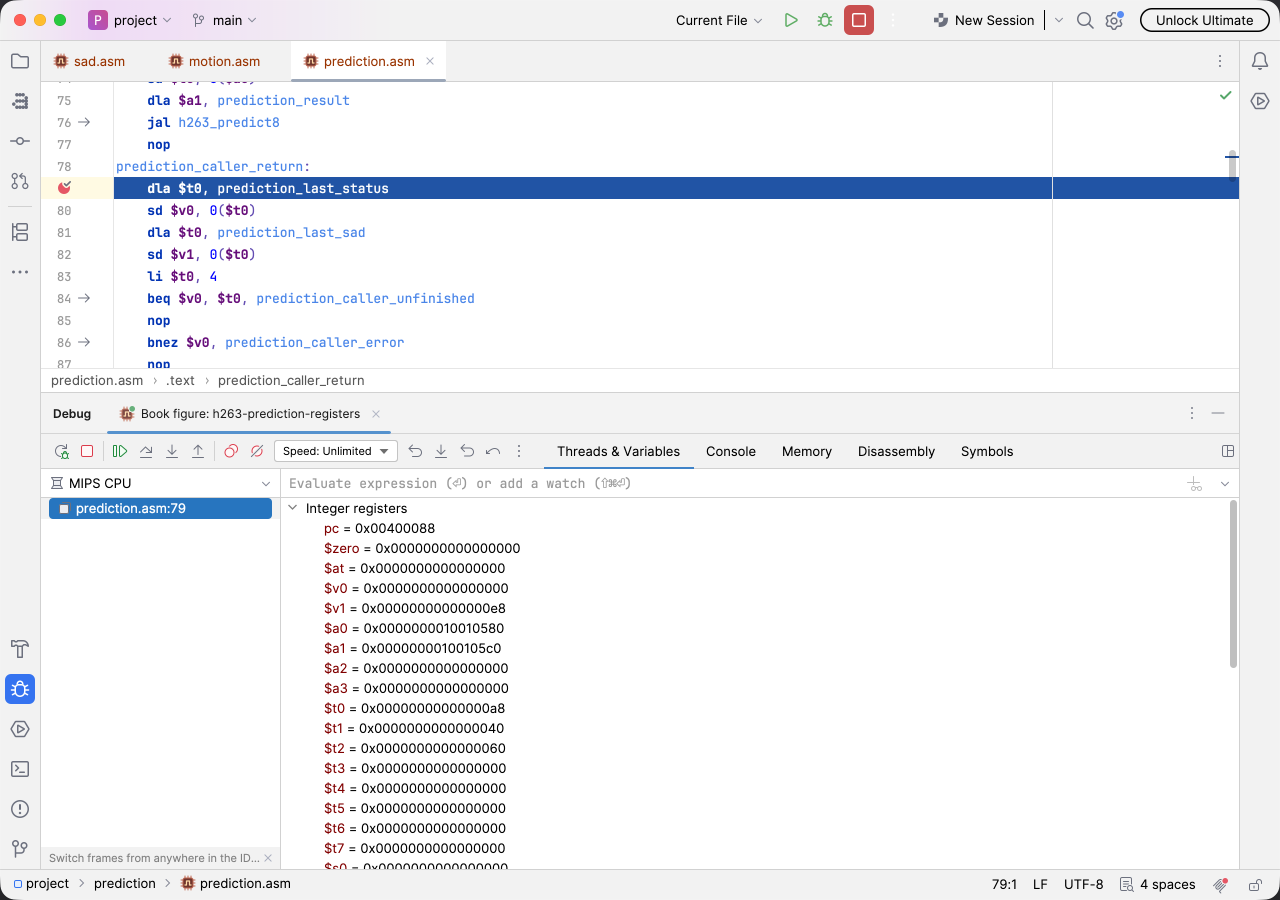
\includegraphics[artifact]{packages/035-h263/captures/h263-prediction-residual/registers.png}}
\sbox2{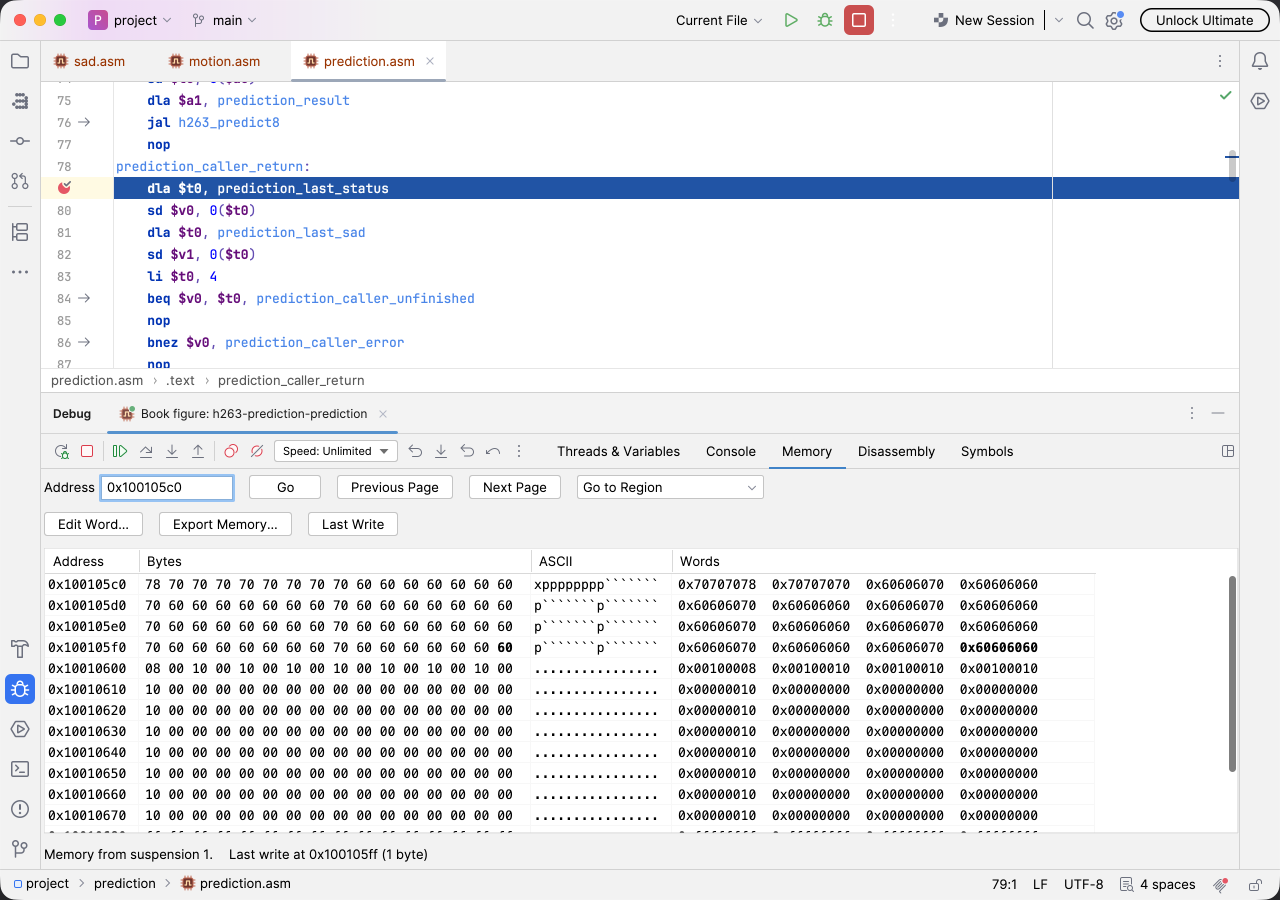
\includegraphics[artifact]{packages/035-h263/captures/h263-prediction-residual/prediction.png}}
\sbox4{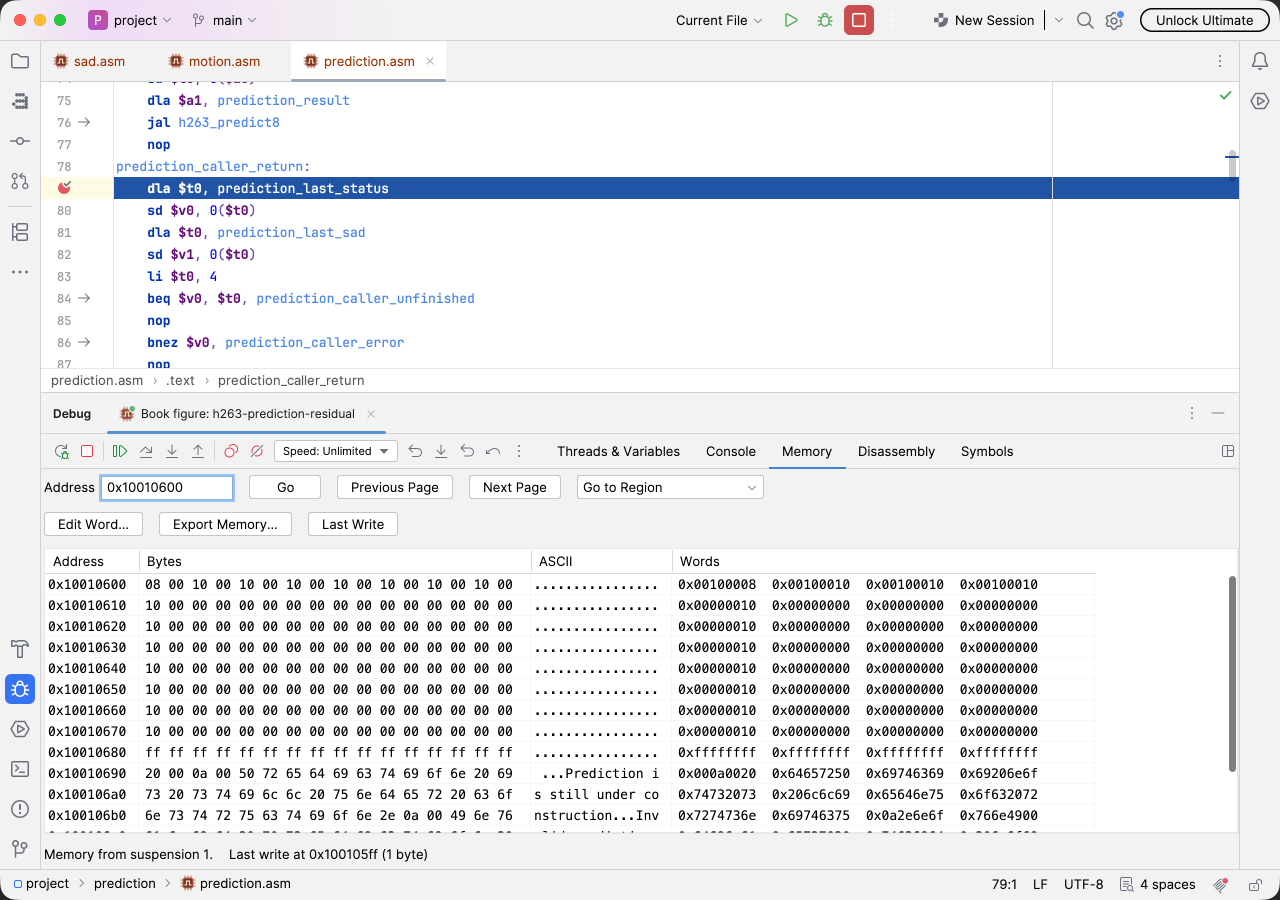
\includegraphics[artifact]{packages/035-h263/captures/h263-prediction-residual/residual.png}}
\edef\MARSpredictionsourceLeft{\the\dimexpr0.036718750\wd0\relax}
\edef\MARSpredictionsourceBottom{\the\dimexpr0.774444444\ht0\relax}
\edef\MARSpredictionsourceRight{\the\dimexpr0.611718750\wd0\relax}
\edef\MARSpredictionsourceTop{\the\dimexpr0.170000000\ht0\relax}
\edef\MARSpredictionpredictionLeft{\the\dimexpr0.108593750\wd2\relax}
\edef\MARSpredictionpredictionBottom{\the\dimexpr0.335555556\ht2\relax}
\edef\MARSpredictionpredictionRight{\the\dimexpr0.585156250\wd2\relax}
\edef\MARSpredictionpredictionTop{\the\dimexpr0.634444444\ht2\relax}
\edef\MARSpredictionresidualLeft{\the\dimexpr0.108593750\wd4\relax}
\edef\MARSpredictionresidualBottom{\the\dimexpr0.335555556\ht4\relax}
\edef\MARSpredictionresidualRight{\the\dimexpr0.585156250\wd4\relax}
\edef\MARSpredictionresidualTop{\the\dimexpr0.634444444\ht4\relax}
\edef\MARSpredictionreturnsLeft{\the\dimexpr0.246093750\wd0\relax}
\edef\MARSpredictionreturnsBottom{\the\dimexpr0.310000000\ht0\relax}
\edef\MARSpredictionreturnsRight{\the\dimexpr0.596875000\wd0\relax}
\edef\MARSpredictionreturnsTop{\the\dimexpr0.638888889\ht0\relax}
\begin{tikzpicture}[alt={Four annotated IDE details at prediction_caller_return. The first prediction byte is 78, decimal 120, followed by 70 and 60 bytes. A separate residual region starts with one little-endian 08 00 halfword, decimal eight, followed by 10 00 halfwords. Register v0 is zero and v1 is e8, decimal 232. The highlighted dla precedes the caller status store.}]
\node[anchor=north west,inner sep=0,font=\small\bfseries] (source-title) at (6mm,0) {Prediction is complete; caller stores are next};
\node[anchor=north west,inner sep=0] (source) at ([yshift=-1mm]source-title.south west) {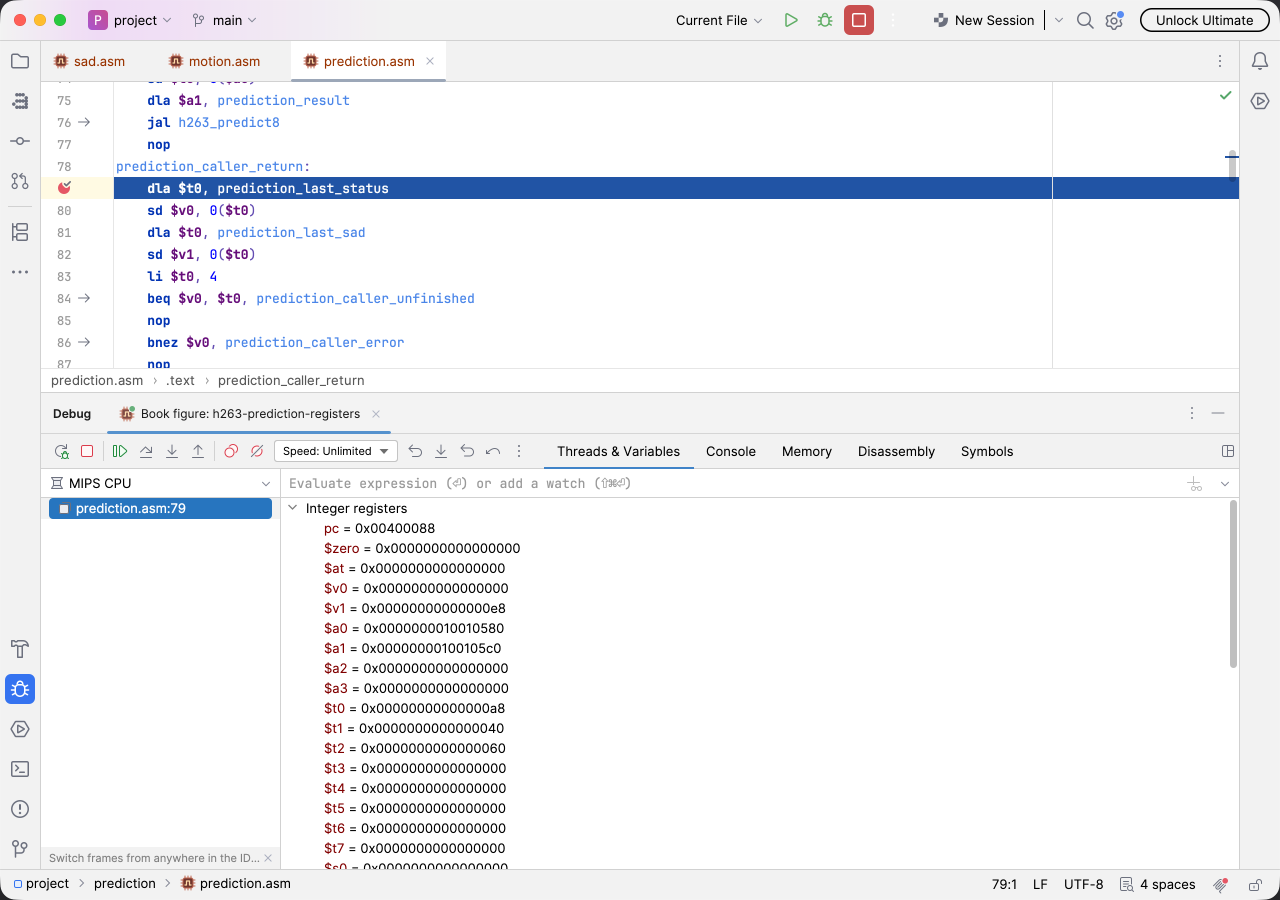
\includegraphics[width=0.7\linewidth,artifact,trim={\MARSpredictionsourceLeft{} \MARSpredictionsourceBottom{} \MARSpredictionsourceRight{} \MARSpredictionsourceTop{}},clip]{packages/035-h263/captures/h263-prediction-residual/registers.png}};
\begin{scope}[shift={(source.south west)},x={($(source.south east)-(source.south west)$)},y={($(source.north west)-(source.south west)$)}]
\draw[black,line width=0.7pt] (0.153333333,0.080000000) rectangle (0.760000000,0.520000000);
\node[draw=black,fill=white,circle,inner sep=1.5pt,font=\footnotesize] at ($(0.153333333,0.520000000)+(-3mm,0)$) {1};
\end{scope}
\node[anchor=north west,inner sep=0,font=\small\bfseries] (prediction-title) at ([yshift=-2mm]source.south west) {Prediction region: unsigned byte samples};
\node[anchor=north west,inner sep=0] (prediction) at ([yshift=-1mm]prediction-title.south west) {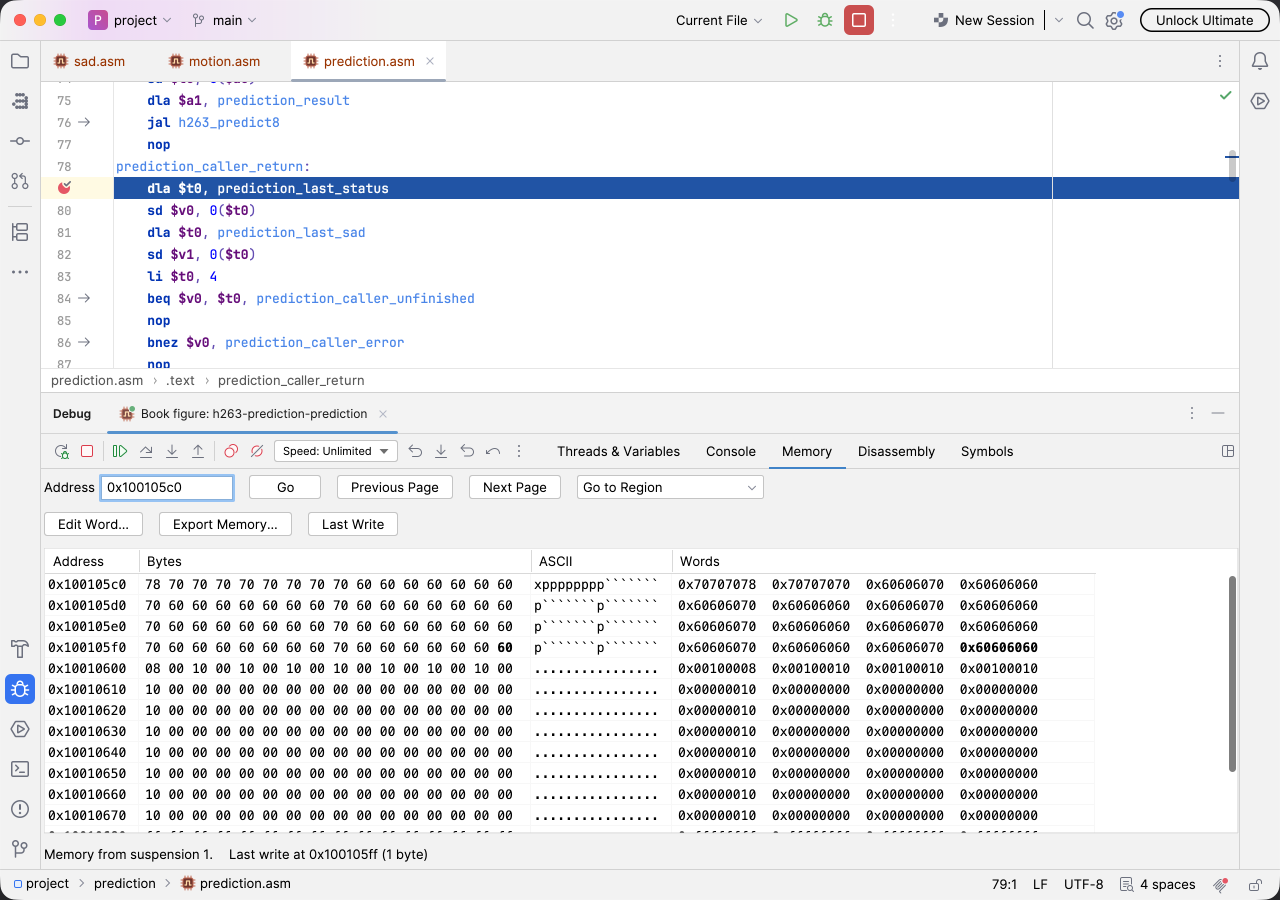
\includegraphics[width=0.84\linewidth,artifact,trim={\MARSpredictionpredictionLeft{} \MARSpredictionpredictionBottom{} \MARSpredictionpredictionRight{} \MARSpredictionpredictionTop{}},clip]{packages/035-h263/captures/h263-prediction-residual/prediction.png}};
\begin{scope}[shift={(prediction.south west)},x={($(prediction.south east)-(prediction.south west)$)},y={($(prediction.north west)-(prediction.south west)$)}]
\draw[black,line width=0.7pt] (0.000000000,0.111111111) rectangle (1.000000000,0.888888889);
\node[draw=black,fill=white,circle,inner sep=1.5pt,font=\footnotesize] at ($(0.000000000,0.888888889)+(-3mm,0)$) {2};
\end{scope}
\node[anchor=north west,inner sep=0,font=\small\bfseries] (residual-title) at ([yshift=-2mm]prediction.south west) {Residual region: signed halfwords};
\node[anchor=north west,inner sep=0] (residual) at ([yshift=-1mm]residual-title.south west) {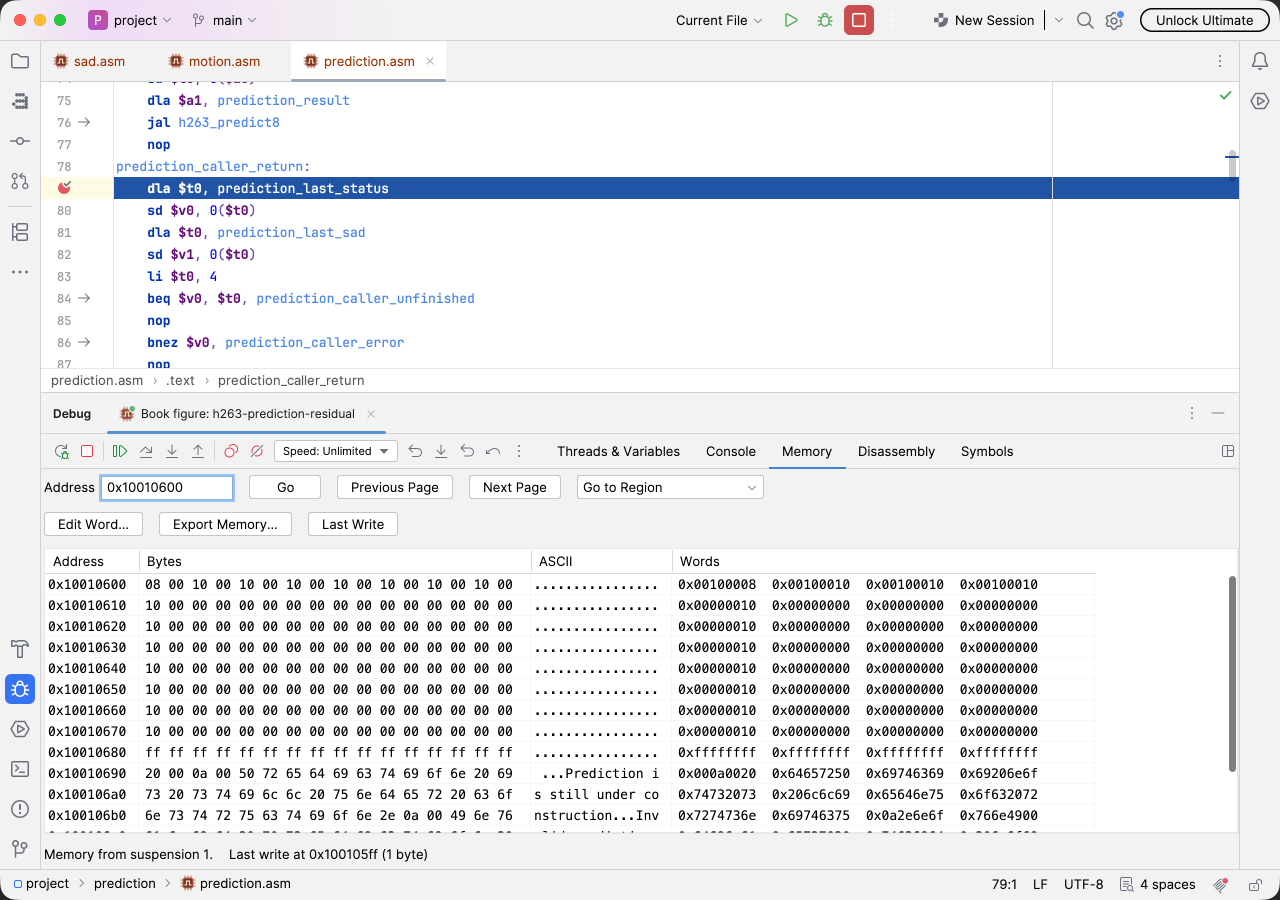
\includegraphics[width=0.84\linewidth,artifact,trim={\MARSpredictionresidualLeft{} \MARSpredictionresidualBottom{} \MARSpredictionresidualRight{} \MARSpredictionresidualTop{}},clip]{packages/035-h263/captures/h263-prediction-residual/residual.png}};
\begin{scope}[shift={(residual.south west)},x={($(residual.south east)-(residual.south west)$)},y={($(residual.north west)-(residual.south west)$)}]
\draw[black,line width=0.7pt] (0.000000000,0.111111111) rectangle (1.000000000,0.888888889);
\node[draw=black,fill=white,circle,inner sep=1.5pt,font=\footnotesize] at ($(0.000000000,0.888888889)+(-3mm,0)$) {3};
\end{scope}
\node[anchor=north west,inner sep=0,font=\small\bfseries] (returns-title) at ([yshift=-2mm]residual.south west) {Successful prediction and residual SAD};
\node[anchor=north west,inner sep=0] (returns) at ([yshift=-1mm]returns-title.south west) {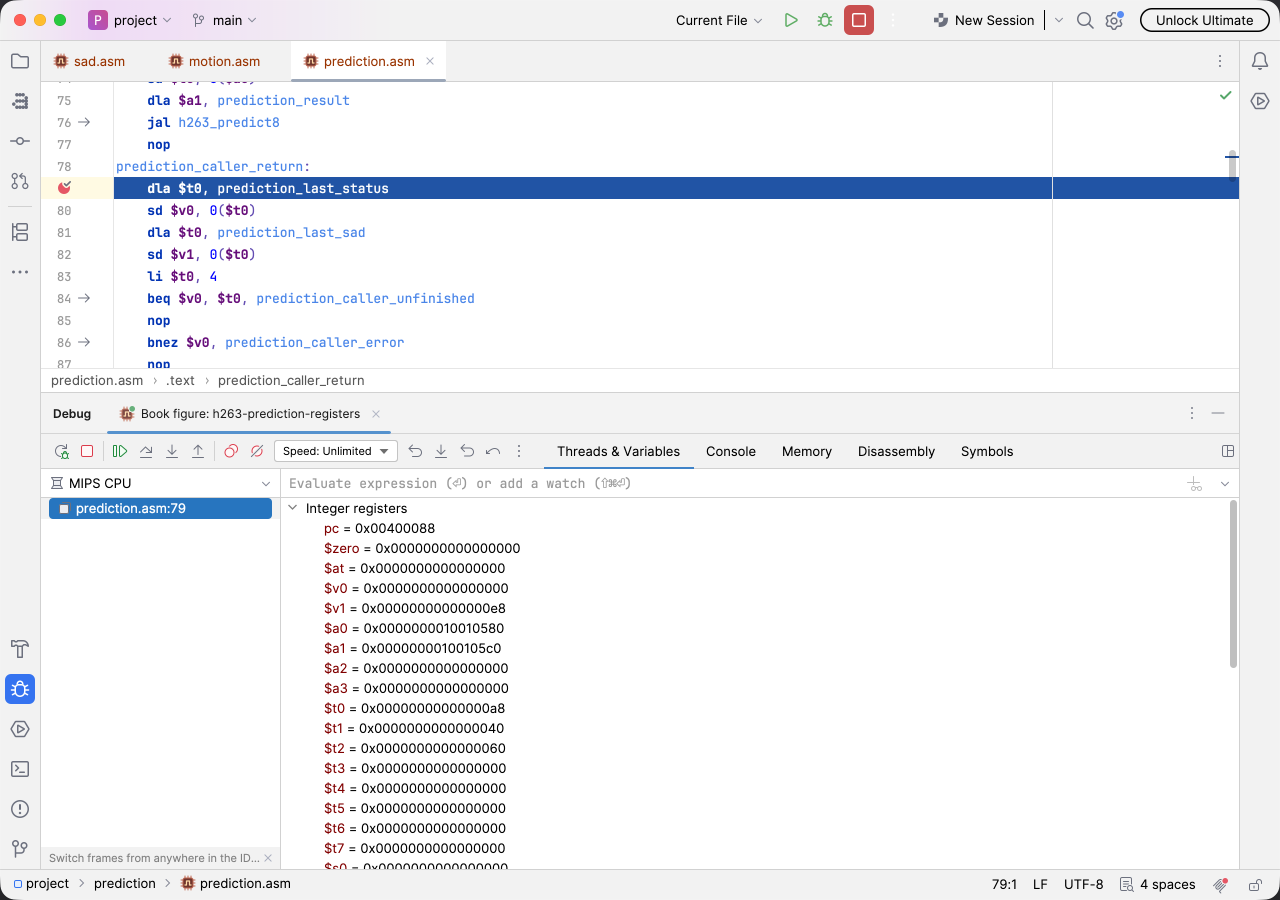
\includegraphics[width=0.5\linewidth,artifact,trim={\MARSpredictionreturnsLeft{} \MARSpredictionreturnsBottom{} \MARSpredictionreturnsRight{} \MARSpredictionreturnsTop{}},clip]{packages/035-h263/captures/h263-prediction-residual/registers.png}};
\begin{scope}[shift={(returns.south west)},x={($(returns.south east)-(returns.south west)$)},y={($(returns.north west)-(returns.south west)$)}]
\draw[black,line width=0.7pt] (0.029850746,0.065217391) rectangle (0.970149254,0.934782609);
\node[draw=black,fill=white,circle,inner sep=1.5pt,font=\footnotesize] at ($(0.029850746,0.934782609)+(-3mm,0)$) {4};
\end{scope}
\end{tikzpicture}
\par\smallskip
\begin{minipage}{\linewidth}
\small
\begin{enumerate}
\item The callable predictor has finished its work. The next \texttt{dla} begins the caller\textquoteright s bookkeeping, so use the returned registers and published result array here.
\item The first sample is \texttt{78} hexadecimal, or 120. This panel shows the first sixteen unsigned prediction bytes; the complete prediction contains 64 samples.
\item Residuals start at result offset 64. Read two bytes per signed halfword: \texttt{08 00} is eight in this little-endian session. The current sample 128 minus prediction 120 gives this positive residual. The following \texttt{10 00} values are 16, not two independent pixel samples.
\item \texttt{\$v0}=0 and \texttt{\$v1}=\texttt{0xe8}=232. The returned SAD sums magnitudes of all 64 signed residuals.
\end{enumerate}
\end{minipage}
\caption{Predicted bytes and signed residual halfwords occupy separate regions. Three Debug launches share the same prepared input and return checkpoint.}
\label{fig:h263-prediction-residual}
\end{figure}
